\documentclass[12pt,a4paper]{report}
\usepackage[francais]{babel}
\usepackage[pdftex]{graphicx}
\usepackage [utf8x]{inputenc}
\usepackage{amsmath}
\usepackage{amsfonts}
\usepackage{amssymb}
\usepackage[colorlinks=true,linkcolor=black,urlcolor=black]{hyperref}
\usepackage{algorithm}
\usepackage{algorithmic}
\usepackage{subfigure}
\renewcommand{\algorithmicrequire} {\textbf{\textsc{Entrées:}}}
\renewcommand{\algorithmicensure}  {\textbf{\textsc{Sorties:}}}
\renewcommand{\algorithmicwhile}   {\textbf{tant que}}
\renewcommand{\algorithmicdo}      {\textbf{faire}}
\renewcommand{\algorithmicendwhile}{\textbf{fin tant que}}
\renewcommand{\algorithmicend}     {\textbf{fin}}
\renewcommand{\algorithmicif}      {\textbf{si}}
\renewcommand{\algorithmicendif}   {\textbf{finsi}}
\renewcommand{\algorithmicelse}    {\textbf{sinon}}
\renewcommand{\algorithmicthen}    {\textbf{alors}}
\renewcommand{\algorithmicfor}     {\textbf{pour}}
\renewcommand{\algorithmicforall}  {\textbf{pour tout}}
\renewcommand{\algorithmicdo}      {\textbf{faire}}
\renewcommand{\algorithmicendfor}  {\textbf{fin pour}}
\renewcommand{\algorithmicloop}    {\textbf{boucler}}
\renewcommand{\algorithmicendloop} {\textbf{fin boucle}}
\renewcommand{\algorithmicrepeat}  {\textbf{répéter}}
\renewcommand{\algorithmicuntil}   {\textbf{jusqu'à}}
\renewcommand{\algorithmicreturn}   {\textbf{retourner}}

\floatname{algorithm}{Algorithme}

\let\mylistof\listof
\renewcommand\listof[2]{\mylistof{algorithm}{Liste des algorithmes}}

\makeatletter
\providecommand*{\toclevel@algorithm}{0}
\makeatother


\title{\Huge{Cours de Courbes Elliptiques}}
\author{Ecrit par Marion Candau \\\\
Enseignant : M.Karim Belabas\\\\\\\\\\\\\
Master 1 Cryptologie et Sécurité Informatique\\
Université Bordeaux 1}
\date{2009 - 2010}


\begin{document}

\maketitle
\tableofcontents
\newpage 

\chapter{Introduction}
Soit G un groupe cyclique engendré par g d'ordre n c'est-à-dire $g^n=g^0$.
Il existe un isomorphisme de groupe entre G et $\mathbb{Z}/n\mathbb{Z}$ défini par :
$$ (G,\times) \longrightarrow (\mathbb{Z}/n\mathbb{Z},+) $$
$$ g^k \longmapsto k $$
\section{Dissymétrie}
La fonction $ k \longmapsto g^k $ se calcule en $ O(\log k) $ dans G.\\
$ \displaystyle k=\sum_{i=0}^{l} \epsilon_i \times 2^i $  avec $\epsilon_i \in \{0,1\}$\\
$\displaystyle g^k=\prod_{i=0}^{l} \left(g^{2^i}\right)^{\epsilon_i} = \prod_{i=0,\epsilon_i=1}^{l} g^{2^i} $\\
Etant donné $h \in G$,on veut $k \in \mathbb{Z}/n\mathbb{Z} $ tel que $ h = g^k $. On a donc un problème de logarithme discret.\\

$ 0 \leqslant k < n $, $m$ paramètre $\simeq \sqrt{n} $\\
$k=k_1\times m + k_0$, avec $0 \leqslant k_0 < m $ et $ 0 \leqslant k_1 \leqslant \frac{k}{m} \leqslant \frac{n}{m} $\\
$g^{k_1 \times m + k_0} = h \Longleftrightarrow (g^m)^{k_1} = h \times g^{-k_0}  $\\
On a :\\
$$ L_1=\{h\times g^{-k_0}:0 \leqslant k_0 < m\} $$
$$ L_2 = \{ (g^m)^{k_1} : 0 \leqslant k_1 < \frac{n}{m} \} $$
\begin{algorithm}
\caption{Algorithme "générique" (méthode de Shanks : pas de bébé, pas de géant)}
\algsetup{
linenosize = \small,
linenodelimiter=.}
\begin{algorithmic}[1]
\STATE Construire $L_1$
\STATE Trier $L_1$
\STATE Successivement chercher $g^0, g^m, g^{2m}, \ldots $ dans $L_1$
\STATE Si $ k_1 \geqslant 0 $ est le plus petit indice tel que $(g^m)^k \in L_1$, on pose $ k=k_0 + k_1\times m $.
\end{algorithmic}
\end{algorithm}
\paragraph{Coût : }
m multiplications dans G $\Longrightarrow L_1$ et $ g^m$ \\
+ au plus $\frac{n}{m}$ multiplications + recherche + tri \\
La valeur de m qui minimise $ m + \frac{n}{m} $ est $ \lfloor \sqrt{n} \rceil $. Dans un modèle ou la multiplication et la comparaison d'éléments de G coûtent 1, le coût total est en $ O(\sqrt{n} \log n) $.
\begin{algorithm}
\caption{Algorithme "générique" (Pohlig-Helmann)}
\begin{algorithmic}
\STATE Soit G cyclique d'ordre n, g d'ordre n, $p|n :n=pq$
\STATE $g^k=h \Longrightarrow (g^p)^k = h^p, g^p $ est d'ordre $ \frac{n}{p}=q$.
\STATE $\Longrightarrow k \in \mathbb{Z}/q\mathbb{Z}$ en résolvant un problème de logarithme discret de taille q : 
\STATE $ k=k_0 + k_1\times q$ où $k_0$ est connu.
\STATE $g^{k_0} \times (g^q)^{k_1} = h \Rightarrow (g^q)^{k_1}=h \times g^{-k_0} $ 
\STATE $\Longrightarrow $ problème de logarithme discret de taille p.
\end{algorithmic}
\end{algorithm}
\paragraph{Définition\\}
$ \tilde{O}(f)=O(f)\times (\log{f})^{O(1)} $
\paragraph{Corollaire\\}
Un logarithme discret de taille n se calcule en $\tilde{O}(\sqrt{p})$ ou p est le plus grand diviseur premier de n.\\
Conséquence : on veut n premier ou premier en petit cofacteur : $$ n = \underset{premier}{p} \times \underset{\leqslant 10}c $$
Remarque : Si $l$ est premier tel que $p=2\times l + 1$ soit premier, on a : $\# F_{p}^{*} = 2l$
\paragraph{Théorème de Shoup\\}
Cette complexité est optimale dans le modèle du groupe générique.
\begin{algorithm}
\caption{Algorithme "non générique" : Calcul d'indice sur $ F_p^*$}
\begin{algorithmic}
\STATE On choisit $\mathcal{B}=\{l \leqslant B : l $ premier$ \}$ ($B=o(p^\epsilon), \forall \epsilon > 0, B $ petit).
\STATE On recherche des relations dans $  F_p^*$ de la forme :
\STATE $\displaystyle g^x \equiv \prod_{l \in \mathcal{B}} l^{e_l(x)} \mod{p} $ avec $ e_l(x) \in \mathbb{N}, x \in \mathbb{N} $
\STATE $ \displaystyle x  \equiv \sum_{l \in \mathcal{B}} e_l(x) \log{l} \mod{p-1} $
\STATE $\displaystyle \Longrightarrow \log{l}, l \in \mathcal{B} $
\STATE On cherche x tel que $ \displaystyle h\times g^x = \prod_{l \in \mathcal{B}} l^{e_l(x)} \mod{p} $
\STATE $ \displaystyle \Longrightarrow \log{h} = \sum_{l \in \mathcal{B}} e_l(x) \log{l} -x $
\end{algorithmic}
\end{algorithm}
\paragraph{Corollaire\\}
On sait résoudre le problème du logarithme discret dans $F_q^*$ en temps $ L_{\frac{1}{2}}(\log{p})^{O(1)} = o(p^\epsilon) $ $ \forall \epsilon > 0$
\paragraph{Conjecture\\}
On peut remplacer par $ L_{\frac{1}{3}}(\log{p})^{O(1)} $.
\chapter{Courbes Elliptiques}
\section{Définitions}
Soit K un corps ($K=\mathbb{R}, \mathbb{F}_q$).\\
On appelle $K^n=K\times \ldots \times K$ l'espace affine de dimension n sur K. \\$ K^n=\{(x_1,\ldots,x_n),x_i \in K\}$.\\
On appelle $(K^{n+1}  \backslash \{(0,\ldots,0)\})/\sim:x\sim y \Leftrightarrow \exists \lambda \in K^*, x= \lambda y $ l'espace projectif de dimension n sur K.
\paragraph{Notation}
On note $(x_0:x_1:\ldots:x_n)$ la classe de\\ $(x_0,x_1,\ldots,x_n) \in K^{n+1}\backslash \{(0,\ldots,0)\}$.\\
L'espace affine est noté $\mathbb{A}^n(K)$.\\
L'espace projectif sera noté $\mathbb{P}^n(K)$.
\paragraph{Remarque\\}
Tous les points $(1:0),\{(x:1),x \in K\} $ sont différents dans $\mathbb{P}^1(K)$. Plus généralement, considérons dans $\mathbb{P}^n(K)$, $(x_0:\ldots:x_n) \in \mathbb{P}^n(K)$
\begin{itemize}
\item Si $x_n=0$, $(x_0:\ldots:x_n) \longleftrightarrow \mathbb{P}^{n-1}(K) $ points à l'infini.
\item Si $x_n \neq 0$, $(x_0:\ldots:x_n)=\left(\frac{x_0}{x_n}: \frac{x_1}{x_n}:\ldots:\frac{x_{n-1}}{x_n}:1\right) \longleftrightarrow \mathbb{A}^n(K) $ points finis
\end{itemize}
D'ou : 
$$ \mathbb{P}^{n}(K)=U^n \amalg U^{n-1} \amalg \ldots \amalg U^0 $$
avec $ U^i=\{ (x_0:\ldots:x_{i-1}:1:0:\ldots:0),x_0,\ldots,x_{i-1} \in K\} $\\
$U^i$ peut s'interpréter comme $K^i = \mathbb{A}^i(K)$
\paragraph{Définition\\}
On appelle courbe plane sur K, une équation du type $\mathcal{C}:C(x,y,z)=0$ ou C est un polynome homogène de $K[x,y,z]$ c'est-à-dire $$\displaystyle C(X,Y,Z)=\sum_{i,j,k}\lambda_{i,j,k} X^i Y^j Z^k $$
\paragraph{Notation\\}
$\mathcal{C}(K)=\{(x:y:z)\in \mathbb{P}^2(K)$ tel que $ C(x,y,z)=0\}$ sont les points de la courbe.
\paragraph{Remarque\\}
$\forall (x,y,z) \in K, C(\lambda x, \lambda y, \lambda z)= \lambda^{cste} \times C(x,y,z) $
\paragraph{Définition\\}
Soit $\mathcal{C}$ une courbe plane définie par $ C(x,y,z) \in K[X,Y,Z] $ avec $L\supseteq K$. $(x:y:z) \in \mathcal{C}(L) \subseteq \mathbb{P}^2(L)$ est non-singulier (ou régulier) si :
$$ \left(
\begin{array}{c}
   \displaystyle \frac{\partial C}{\partial X} \\
   \\
    \displaystyle\frac{\partial C}{\partial Y}  \\
    \\
   \displaystyle \frac{\partial C}{\partial Z} 
\end{array}
\right)\times (x,y,z) \neq \left(
\begin{array}{c}
   \displaystyle 0 \\
   \\
    \displaystyle 0  \\
    \\
   \displaystyle 0 
\end{array}
\right)$$
\paragraph{Définition\\}
Soit $\mathcal{E}:(YZ^2+a_1XYZ+a_3YZ^2)-(X^3+a_2X^2Z+a_4XZ^2+a_6Z^3)$ avec $(a_1,a_2,a_3,a_4,a_6) \in K $.\\
$\mathcal{E}$ est une cubique plane projective sur un corps K.
\paragraph{Remarque\\}
$\mathcal{E}(K) \neq 0$ et $(0:1:0) \in \mathcal{E}(K)$ c'est le seul point à  l'infini de $\mathcal{E}(K)$
\paragraph{Définition\\}
Soit $\bar{K} \supset K$ une cloture algébrique de K. $\mathcal{E} $ est dite singulière si tous les points de $\mathcal{E}(\bar{K})$ sont non-singuliers. Une cubique comme ci-dessus est appelée courbe elliptique. 
\paragraph{Cas particulier (important)\\}
La forme courte de Weierstass est définie par : $a_1=a_2=a_3=0 $. La courbe a donc l'équation suivante :
$$ \mathcal{E} : Y^2Z=X^3+aXZ^2+bZ^3 $$
$ \mathcal{E}$ est non singulière $ \Longleftrightarrow $ le polynome cubique $ X^3+aX+b$ n'a pas de racine double 
$\Longleftrightarrow -4a^3+27b^2 \neq 0 $
\paragraph{Remarque\\}
Si $car(K)\neq 2,3$, toute courbe elliptique se ramène  à une équation de Weierstrass (par un changement de variable simple).
\paragraph{Définition + théorème\\}
On pose $0=(0:1:0) \in \mathcal{E}(K)$. \\
Si $P=(x:y:1)\in \mathcal{E}(K)$, on pose $\ominus P = (x:-a_1x-a_3-y:1)\in \mathcal{E}(K)$.\\
Soient $P_1=(x_1:y_1:1)$ et $P_2=(x_2:y_2:1) \in \mathcal{E}(K), P_1 \neq \ominus P_2$.\\
Soit $ m =  \left\{
    \begin{array}{ll}
        \displaystyle \frac{y_1-y_2}{x_1-x_2} & \mbox{si } P_1 \neq P_2 \\
        \\
        \displaystyle \frac{3x_1^2+2a_2x_1+a_4-a_1y_1}{2y_1+a_1x_1+a_3} & \mbox{sinon.}
    \end{array}
\right.$ \\ \\
$$P3= \left\{
	\begin{array}{l}
        \displaystyle  x_3=-x_1-x_2-a_2+m(m+a_1)\\
        \\
        \displaystyle y_3=-y_1-a_3-a_1x_3+m(x_1-x_3) 
    \end{array}
\right.$$\\
On pose $P_1 \oplus P_2 =P_3 = (x_3:y_3:1) \in \mathcal{E}(K) $. $(\mathcal{E}(K) ,\oplus)$ est un groupe abélien, de neutre 0 et d'inverse donné par $P \longmapsto \ominus P $.
\begin{figure}[htp]
  \centering
  \caption{Dessin si $K=\mathbb{R}$ de la partie affine de la courbe $y^2=x^2+ax+b$}
  \subfigure[$\delta > 0$]{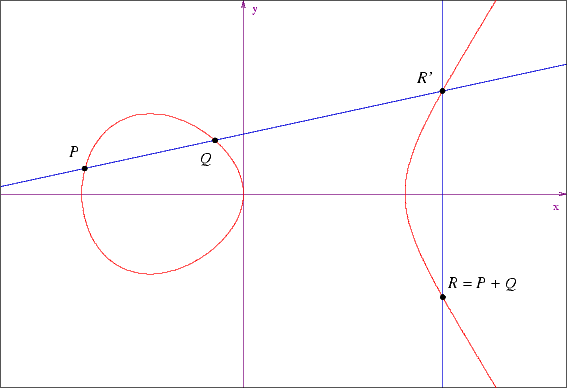
\includegraphics[width=0.6\textwidth]{courbe1.png}}                
  \subfigure[$\delta <0$]{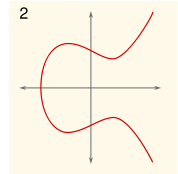
\includegraphics[width=0.3\textwidth]{courbe2.png}} \\
\end{figure}
\paragraph{Notation\\}
Pour $n \in \mathbb{Z}$, $P \in \mathcal{E}(K)$, on pose : \\
$$[n] P = \left\{
	\begin{array}{ll}
        \displaystyle  P\oplus P \oplus P \oplus \ldots \oplus P & \mbox{si } n > 0\\
        0 & \mbox{si } n=0 \\
        \displaystyle [-n](\ominus P) & \mbox{si } n < 0 
    \end{array}
\right.$$
C'est la multiplication scalaire sur $\mathcal{E}$.
\paragraph{Théorème : borne de Hasse}
$$ \left| \# \mathcal{E}(\mathbb{F}_q)-(q+1) \right| \leqslant 2\sqrt{q} \Longrightarrow \left| \# \mathcal{E}(\mathbb{F}_q^k)-(q^k+1) \right| \leqslant 2 q^{\frac{k}{2}} $$
$ \# \mathcal{E}(\mathbb{F}_q) = q^k + 1 - \alpha^k - \beta^k $ où $\alpha, \beta $ sont les racines complexes d'une équation $X^2 -sX + q =0 $ tel que $ |\alpha | = |\beta | = \sqrt{q} $ et $\alpha + \beta = s $ et $ \alpha \beta =q$.

\paragraph{Problèmes\\}
\begin{itemize}
\item Divisions : couteux sur un processeur dédié
\begin{itemize}
\item[$\rightarrow$] coordonnées projectives : $ (x:y:z) = (\frac{x}{z}:\frac{y}{z}:1)$
\item[$\rightarrow$] formules polynomiales pour $(x_3,y_3,z_3)=P_3=P_1\oplus P_2$ en termes de $(x_1:y_1:z_1) = P_1 $ et $(x_2:y_2:z_2)=P_2$ plus rapide que la loi de groupe sur la forme de Weierstrass.
\end{itemize}
\item Side Channel Attacks (SCA) / Attaques par canaux cachés $ \rightarrow $ Attaques physiques $\Longrightarrow$ 
Formules unifiées : on rajoute des opérations fictives dans les deux sous-opérations atomiques $ \longrightarrow $ indistinguables.
\end{itemize}
\paragraph{Courbes d'Edwards\\}
$\mathcal{C}(K) : x^2 + y^2 = c^2(1+dx^2y^2), c,d \in K, car(K) \neq 2 $\\
Soient $ P_1 = (x_1,y_1)$ et $ P_2=(x_2,y_2)$. On a :
$$ P_3 = P_1 \oplus P_2 = \left( \frac{x_1y_2+x_2y_1}{c(1+dx_1x_2y_1y_2)},\frac{y_1y_2-x_1x_2}{c(1-dx_1x_2y_1y_2)}\right) \in \mathcal{C}(K) $$
En général, c et d sont petits.
\paragraph{Théorème\\}
$\oplus$ est une loi de groupe sur $ \mathcal{C}(K)$ de neutre $(0,c)$ et d'inverse \\$\ominus (x,y) = (-x,y)$.
\paragraph{Remarque\\}
$(0,-c)$ est d'ordre 2, $(-c,0)$ est d'ordre 4.
\paragraph{Théorème\\}
Soit $e=1-dc^4$ avec d non carré et $ e \neq 0$, et $$\displaystyle E:\frac{1}{e} Y^2 = X^3 + \left(\frac{4}{e}-2\right) X^2 + X $$ Pour $i=1,2,3$ on définit $ Q_i$ de la façon suivante :
\begin{itemize}
\item[$\circ$] $Q_i = 0 $ si $(x_i,y_i)=(0,c)$
\item[]
\item[$\circ$] $Q_i=(0,0) $ si $ (x_i,y_i) = (0,-c)$
\item[]
\item[$\circ$] $ \displaystyle Q_i=\left(\frac{c+y_i}{c-y_i},\frac{2c(c+y_i)}{(c-y_i)x_i}\right)$ si $ x_i \neq 0 \Rightarrow y_i \neq c$
\item[]
\end{itemize}
Alors $ Q_i \in E(K) $ et $ Q_3 = Q_1 + Q_2$.
\paragraph{Addition efficace\\}
$$ (X^2 + Y^2)Z^2 - c^2 (Z^4 + dX^2Y^2)$$
$$ (X:Y:Z) \longmapsto \left(\frac{X}{Z},\frac{Y}{Z}\right) \mbox{ sur la courbe affine avec } Z \neq 0$$
$$ (X_1:Y_1:Z_1) \oplus (X_2:Y_2:Z_2) = (X_3:Y_3:Z_3)$$
\begin{enumerate}
\item $A \leftarrow Z_1Z_2$\\
$ B \leftarrow A^2$\\
$C \leftarrow X_1X_2 $ \\
$ D \leftarrow Y_1Y_2 $ \\
$ E \leftarrow d C D $\\
$ F \leftarrow B-E$\\
$G \leftarrow B+E $
\item $ X_3 \leftarrow AF((X_1+Y_1)(X_2+Y_2)-C-D)$\\
$ Y_3 \leftarrow AG(D-C)$\\
$Z_3 \leftarrow cFG$
\end{enumerate}
Coût total : 10 multiplications + 1 mise au carré + 1 multiplication par c + 1 multiplication par d + 7 additions
\paragraph{Espace\\}
$(R_1,R_2,R_3) \rightarrow P_1 $ et $ (R_4,R_5,R_6) \rightarrow P_2 $: 2 registres pour calculer\\ $P_1 \leftarrow P_1 \oplus P_2 $\\
On a environ : mise au carré $\approx 0,7 $ multiplications, multiplications par c $\approx$ multiplications par d $\approx $ additions.
\paragraph{2 cas particuliers\\}
\begin{enumerate}
\item $Z_1=1$
\item Doublement $P_1=P_2$ 3 multiplications + 4 mises au carré + 3 multiplications par c + 6 additions
\end{enumerate}
\chapter{Comptage de points}
On cherche   calculer le cardinal de $E(\mathbb{F}_q) $. Le but est de garantir que $\# E(\mathbb{F}_q) $ n'est pas friable, idéalement est premier ($\# E(\mathbb{F}_q) = \underset{\leqslant 4}{c} \times \underset{premier}{l}$).
\paragraph{Remarque\\}
Si E est associée  à une courbe d'Edwards, $ 4 | \# E(\mathbb{F}_q) $. \\Si $ E:Y^2 = X^3+aX+b$ telle que $ X^3 +aX+b$ a une racine dans $\mathbb{F}_q $ alors $2 | \# E(\mathbb{F}_q) $.\\Si $ E:Y^2 = X^3+aX+b$ telle que $ X^3 +aX+b$ a 3 racines dans $\mathbb{F}_q $ alors $4 | \# E(\mathbb{F}_q) $.
\paragraph{Deux approches\\}
\begin{enumerate}
\item $E/\mathbb{F}_q $ étant donnés, calculer $\# E(\mathbb{F}_q) $.
\item Etant donnés m tel que $ |m-(q+1)| < 2\sqrt{q}$, construire $ E / \mathbb{F}_q $ tel que $ \# E(\mathbb{F}_q) = m$
\end{enumerate}
\section{Comptage de points général}
On a : car $\mathbb{F}_q \neq 2,3$, $E:Y^2=X^3 +aX+b$.
\paragraph{Définition : Symbole de Legendre\\}
Dans $ \mathbb{Z}/p\mathbb{Z} $, $p\neq 2$, il existe x tel que :
$$ x^{\frac{p-1}{2}}= \left\{\begin{array}{ll}
1 & \Longleftrightarrow \mbox{ x est un carré dans } \mathbb{F}_p^* \\
0 & \Longleftrightarrow x=0 \\
-1 & \Longleftrightarrow \mbox{ x n'est pas un carré}\end{array}\right.$$
On définit le symbole de Legendre : $$ \left(\frac{x}{p}\right) = \left\{\begin{array}{ll}
1 & \Longleftrightarrow \mbox{ x est un carré dans } \mathbb{F}_p^* \\
0 & \Longleftrightarrow x=0 \\
-1 & \Longleftrightarrow \mbox{ x n'est pas un carré}\end{array}\right. \Rightarrow \left(\frac{x}{p}\right) \equiv x^{\frac{p-1}{2}} \mod p $$
\paragraph{Mthode "naïve"\\}
$$\# E(\mathbb{F}_q) = 1 + \sum_{x \in \mathbb{F}_q} \# \{y \in \mathbb{F}_q,y^2 = x^3 +ax+b\}$$
\paragraph{Cas particulier\\}
q premier, q=p.
$$\# E(\mathbb{F}_q) = p+1 + \sum_{x \in \mathbb{F}_p} \left(\frac{x^3+ax+b}{p}\right)$$
\paragraph{Cas général\\}
x est un carré si et seulement si $\displaystyle x^{\frac{q-1}{2}}=1 \Leftrightarrow x^{(p^{e-1}+\ldots+ 1)\left(\frac{p-1}{2}\right)} =1  \Leftrightarrow x^{p^{e-1}+\ldots+ 1} = y \in \mathbb{F}_p$.\\
$$ \# E(\mathbb{F}_q) = q+1 + \sum_{x \in \mathbb{F}_q} \left(\frac{(x^3+ax+b)^{p^{e-1}+\ldots+1}}{p}\right)$$
L'algorithme "naïf" est en $ \tilde{O}(q)$.\\
L'algorithme de Shanks-Mestre est en $ \tilde{O}(q^{\frac{1}{4}})$.
Il utilise : 
\begin{itemize}
\item la borne de Hasse : $ |\# E(\mathbb{F}_q)  -(q+1) | < 2 \sqrt{q} $.
\item S'il existe P d'ordre o dans $E(\mathbb{F}_q) $ alors $ o | \# E(\mathbb{F}_q) $
\end{itemize}
$ \Longrightarrow $ si $ o \geqslant 4\sqrt{q} $ alors $\# E(\mathbb{F}_q) $ est déterminé.
\paragraph{Théorème de Mestre\\}
Soient $ E/\mathbb{F}_q : y^2 = x^3+ax+b$ et $ E'/\mathbb{F}_q : y^2g=x^3+ax+b$ avec $g \not \in (\mathbb{F}_q)^2 $ (tordue quadratique de E)
\begin{itemize}
\item $\# E(\mathbb{F}_q)  + \# E'(\mathbb{F}_q) = 2(q+1)$
\item Si $q \geqslant 229$, il existe $P\in E(\mathbb{F}_q) \cup E'(\mathbb{F}_q)$ dont l'ordre vérifie $o > 4\sqrt{q}$ 
\end{itemize}

Soit $P \in E(\mathbb{F}_q)$, on tire $ x \in \mathbb{F}_q$, si $ x^3+ax+b \in \mathbb{F}_q^2$, on calcule $y$. On veut calculer l'ordre de P. Mais on va faire mieux, on va calculer un multiple x de l'ordre de P tel que $ |x-(q+1)| < 2\sqrt{q} $ (un tel multiple existe, par exemple, $\# E(\mathbb{F}_q) $).
$$ \exists x \mbox{ tel que } [q+1-x]P = 0 \mbox{ (*), } x=x_0+mx_1, 0 \leqslant x_0 <m \mbox{ et } |x_1| < \frac{2\sqrt{q}}{m}+1$$
On choisit m tel que $ m^2 \simeq 4\sqrt{q} \Rightarrow m=\lfloor 2q^{\frac{1}{4}} \rfloor $.
$$ (*) \Leftrightarrow [q+1-x_0]P=[x_1]([m]P)$$
On détermine $x_0,x_1 = O(q^{\frac{1}{4}}) $ tel que (*) vrai.
\begin{algorithm}
\caption{}
\algsetup{
linenosize = \small,
linenodelimiter=.}
\begin{algorithmic}[1]
\REQUIRE $P \in E(\mathbb{F}_q)$
\ENSURE ordre de P
\STATE $ m \leftarrow \lfloor 2q^{\frac{1}{4}} \rfloor $
\STATE On énumère $ L = \{[q+1-x_0]P, 0 \leqslant x_0 < m\} $
\STATE $Q \leftarrow [m]P $\\
Pour tout $x_1$ tel que $ |x_1| < \frac{2\sqrt{q}}{m}+1$, vérifier si $ [x_1]Q $ est dans L.
\STATE $ r \leftarrow q+1 - (x_0 + mx_1) $ est un multiple de l'ordre de P. On factorise r et on calcule l'ordre exact.
\end{algorithmic}
\end{algorithm}

\begin{algorithm}
\caption{Algorithme générique de calcul de l'ordre de P}
\begin{algorithmic}[1]
\REQUIRE $\displaystyle g \in G, r = \prod_{i=1,p_i \mbox{ }premier}^{\omega}p_i^{e_i}$ tel que $ g^r =1$
\ENSURE ordre de g
\FOR{$i=1$à$\omega$}
\STATE $g_i \leftarrow g^{\frac{r}{p_i^{e_i}}}$ est d'ordre divisant $p_i^{e_i}$.
\STATE Soit $f_i$ l'entier minimal tel que $ g_i^{p_i^{f_i}} = 1$, $ f_i < e_i$
\ENDFOR
\STATE Renvoyer $ o =\displaystyle \prod_{i=1}^{\omega} p_i^{f_i} $
\end{algorithmic}
\end{algorithm}
\section{Algorithme de Schoof en $(\log q)^{O(1)}$}
\paragraph{Théorème}
Soit $ E / \mathbb{F}_q$. Si $\# E(\mathbb{F}_q) = q+1-a_q \mbox{ } (a_q \in \mathbb{Z},|a_q| \leqslant 2\sqrt{q})$ alors l'opérateur de Frobenius $$ \phi : E(\bar{\mathbb{F}_q}) \longrightarrow E(\bar{\mathbb{F}_q})$$
$$ (x:y:z) \longmapsto (x^q:y^q:z^q) $$
vérifie l'équation : $ \phi^2-[a_q]\phi+q=0$ c'est-à-dire :
$$ \forall P \in E(\bar{\mathbb{F}_q}), \phi(\phi(P)) \ominus [a_q]\phi(P) \oplus [q]P = 0 \mbox{ (*)} $$

\paragraph{Remarque\\}
$\phi$ est bien définie ! Si$(x:y:z)$ vérifient une équation polynmiale dans $\mathbb{F}_q[X,Y,Z]$ alors $(x^q:y^q:z^q)$ vérifient la même équation\\ $ C(x^q,y^q,z^q) = C(x,y,z)^q = 0$.
\paragraph{Ide de Schoof}
\begin{itemize}
\item Calculer $ a_q \mod l$ pour un grand nombre de petits premiers $l$ tel que $ \prod l_i > 4 \sqrt{q}$ $(\Rightarrow a_q \in \mathbb{Z})$.
\item Soit $E[l]=\{P \in E(\bar{\mathbb{F}_q}) \mbox{ tel que } [l]P=0\}$\\
On choisit P d'ordre $l$ premier dans $E[l]$ et on applique (*). $\phi(P)$ et $\phi^2(P)$ sont aussi d'ordre $l$.\\
On cherche $0 \leqslant \alpha_l < l$ tel que $[\alpha_l]\phi(P) = \phi^2(P) \oplus [q]P$ en $O(l)$ additions alors $ a_q \equiv \alpha_l \mod l$
\item $\displaystyle \sum_{l_i \mbox{ } premier, l_i<x} \ln l_i \sim x > 0,98 x$ pour $ x> 10^6$\\
$ \Rightarrow \displaystyle \sum_{l_i <x}\ln l_i > \ln (4\sqrt{q}) \Rightarrow x \asymp \log \sqrt{q} $
\end{itemize}
\paragraph{Définition : polynomes de n-division\\}
Soit $E/K$, $car(K) \neq 2$.
$$ y^2 + a_1 xy + a_3 y = x^3 + a_2 x^2+ a_4 x + a_6 $$
On pose : $$ b_2=a_1^2 + 4 a_2$$
$$ b_4 = 2a_4+a_1a_3$$
$$b_6 = a_3^2 + 4a_6$$
$$ b_8 = a_1^2 a_6 - a_1a_3a_4 + 4a_2a_6 + a_2a_3^2 -a_4^2$$
Pour la forme courte $y^2 = x^3 +a_4x+a_6 $ on a : $$ b_2=0$$ $$ b_4 = 2a_4$$ $$ b_6=4a_6$$ $$b_8=-a_4^2$$
Ensuite on pose :
$$ f_0(x) = 0 $$
$$f_1(x) = 1$$
$$ f_2(x) = 1$$
$$ f_3(x) = 3x^4 + b_2 x^3 + 3b_4x^2 + 3b_6 x + b_8$$
$$ f_4(x) = 2x^6+b_2x^5+5b_4x^4+10b_6x^3+10b_8x^2+(b_2b_8-b_4b_6)x+(b_4b_8-b_6^3)$$
On pose : $ g(x)= 4x^3+b_2x^2+2b_4x+b_6$\\
Pour $n \geqslant 2$, on définit :
$$f_{2n}=f_n(f_{n+2}f_{n-1}^2-f_{n-2}f_{n+1}^2)$$
$$f_{2n+1}=\left\{\begin{array}{ll}
gf_{n+2}f_n^3-f_{n-1}f_{n+1}^3 & \mbox{ si n pair} \\
f_{n+2}f_n^3-g^2f_{n-1}f_{n+1}^3 & \mbox{ si n impair}
\end{array}\right.$$

\paragraph{Théorème\\}
Si $P=(x,y) \in E[\bar{K}]\setminus E[2]$ alors $P \in E[n] $ si et seulement si $f_n(x)=0$.
\paragraph{Corollaire\\}
Pour trouver $P=(x,y) \in E[l]$ d'ordre l premier, il suffit de résoudre $f_l(x)=0$.\\
Problème : degré $ f_n \asymp n^2$. La solution est Schoof Elkies-Atkin (SEA).
\paragraph{Mthode duale\\}
Connaissant $\#E(\mathbb{F}_q)$ trouver q et E.\\
\begin{enumerate}
\item Soit q puissance d'un premier tel que $$ |q+1-m| \leqslant 2\sqrt{q}$$
$$ \Leftrightarrow -2\sqrt{q} \leqslant q+1-m \leqslant 2\sqrt{q} $$
$$\Leftrightarrow (\sqrt{q}+1)^2 \geqslant \sqrt{m} \geqslant (\sqrt{q}-1)^2$$
$$ \Leftrightarrow -1 \leqslant \sqrt{m}-\sqrt{q} \leqslant 1$$
Problème : il n'est pas certain qu'un tel $q=p^n$, p premier, existe.
\item Théorème \\
Si $|m-(q+1)| < 2\sqrt{q}$, il existe $E / \mathbb{F}_q$, $\#E(\mathbb{F}_q) = m $ (on sait même dire combien de telles E existent).
\item Construction de $E / \mathbb{F}_q$,  $\#E(\mathbb{F}_q) = m $\\
Théorie de la multiplication complexe (CM) $ \mathbb{C} \longrightarrow \mathbb{F}_q $
\begin{enumerate}
\item Pour $ \tau \in h=\{\tau \in \mathbb{C}, Im(\tau) > 0 \}$, on pose $$ q=e^{2i\pi \tau} = \underset{\mbox{module 1}}{e^{2i\pi Re(\tau)}}\times \underset{\in ]0,1[}{e^{-2\pi Im(\tau)}}$$
On pose : 
$$ j(\tau)=1728\times \frac{g_2^3}{g_2^3-27g_3^2} $$
ou : $$ g_2(\tau)=1+240\times \sum_{n\geqslant 1} \frac{n^3q^n}{1-q^n} \in \mathbb{C} $$
$$ g_3(\tau)=1+504 \times \sum_{n\geqslant 1}\frac{n^5q^n}{1-q^n} \in \mathbb{C} $$
\item Courbes elliptiques sur $\mathbb{C}$\\
$E/\mathbb{C} = \mathbb{C} / \Lambda$ ou $\Lambda = \mathbb{Z} + \tau \mathbb{Z} = \{a+b\tau,(a,b)\in \mathbb{Z}^2\}$. C'est un groupe additif, quotient de $(\mathbb{C},+)$.
$$\phi : \mathbb{C}/\Lambda \longrightarrow E[\mathbb{C}]$$
$$ z \longmapsto \left\{\begin{array}{ll}
(p(z):p'(z):1) & \mbox{ si }z  \not\in \Lambda \\
(0:1:0) & \mbox{ si } z \in \Lambda \end{array}\right.$$
$E[\mathbb{C}] = \{(x:y:z) \in \mathbb{P}^2(\mathbb{C})$ vérifient une équation du type $ y^2z=4x^3-G_2xz^2-G_3z^3\}$\\
Théorème :$\phi$ est un morphisme $ (\mathbb{C}/\Lambda, + ) \rightarrow (E(\mathbb{C}),\oplus)$.
\item On peut définir 
$$ J(E_{\tau})=1728\times \frac{G_2^3}{G_2^3-G_3^2}=j(\tau) $$
Soit $j \in K$ corps (car K $\neq $ 2,3), on veut trouver $E/K$ sous forme courte de Weierstrass tel que $J(E)=j$.
\begin{itemize}
\item si $j=0$, $ y^2=x^3-1$
\item si $j=1728$, $y^2=x^3-x$
\item si $j\neq 1728$ et $j\neq 0$, $y^2=x^3+3cx +2c $ ou $c=\frac{j}{1728-j}$
\end{itemize}
$\Longrightarrow J(E)=j$
\item Groupes de classes : soit $D<0$, $D\in \mathbb{Z}$ fixé, on considère \\
$Cl(D)=\{(a,b,c)\in \mathbb{Z}^3$ tel que $ b^2-4ac = D $ et $ |b|\leqslant a \leqslant c, b\geqslant 0 $ si $ a=|b| $ ou $ a=c\}$\\
On a : $ 4ac-b^2 = |D| \geqslant 3a^2 \Rightarrow |a| \leqslant \sqrt{\frac{|D|}{3}} \Rightarrow Cl(D)$ est fini.
Théorème : $\# Cl(D) = \tilde{O}(|D|^{\frac{1}{2}})$\\
\begin{algorithm}[h]
\caption{Algorithme d'énumération de $Cl(D)$}
\begin{algorithmic}[1]
\FOR{$a=1$à$\sqrt{\frac{|D|}{3}}$}
\FOR{$b=0$à$a$ tel que $b=D \mod 2$}
\STATE $c\longleftarrow \frac{b^2-D}{4a}$
\STATE Si $ c \not \in \mathbb{Z}$ ou $ c<a$, on stoppe cette itération et on passe au suivant.
\STATE Afficher $(a,b,c)$
\STATE Si $ b\neq a \neq c$ et $ b\neq 0$, afficher $(a,-b,c)$
\ENDFOR
\ENDFOR
\end{algorithmic}
\end{algorithm}
\item Soit $\displaystyle H(X) = \prod_{a,b,c \in Cl(D)}\left(X-j\left(\frac{-b+\sqrt{D}}{2a}\right)\right) $.\\ En fait, $H(X) \in \mathbb{Z}(X)$, il est facilement calculable.\\
Soit p premier $>3$ tel que l'équation (*) $ U^2-DV^2 = 4p$ ait des solutions entires $(U,V) \in \mathbb{Z}^2$. Alors $\bar{H}(X) \in \mathbb{F}_p[X]$ est scindé.\\
Soit $ j \in \mathbb{F}_p$ une racine de $\bar{H}$ et $E / \mathbb{F}_p $ une courbe elliptique telle que $ J(E)=j$. Alors $ \# E(\mathbb{F}_p)= p+1-U$ pour un U solution de (*).
\end{enumerate}
\end{enumerate}
Soit p premier, $D < 0 \rightarrow Cl(D)$ avec $\# Cl(D) \approx \sqrt{|D|}$.
\begin{enumerate}
\item Hypothèse : $ U^2-DV^2 = 4p, U,V \in \mathbb{Z} (*)$. Remarque : si $D < -4$, il y a au plus deux U solutions (opposés).
\item $ \displaystyle H(X) = \prod_{(a,b,*)\in Cl(D)} \left(X-j\left(\frac{-b + \sqrt{D}}{2a}\right)\right) \in \mathbb{Z}[X]$
\item $\bar{H}$ est scindé sur $ \mathbb{F}_p$ : $\displaystyle \bar{H}(X)=\prod_{i=1}^{dH}(X-\bar{j})$.
\item Soit $E/\mathbb{F}_p$ tel que $j(E) = \bar{j}$ une racine de $\bar{H}$. Alors $\# E(\mathbb{F}_p)=p+1-U$ où U est solution de $(*)$.
\end{enumerate}
\paragraph{Rappel\\}
Si $ E : y^2 = x^3 + ax +b $ a $p+1-U$ points sur $\mathbb{F}_p$ alors sa tordue quadratique $ \tilde{E} : gy^2= x^3 +ax +b $ a $p+1+U$ points sur $\mathbb{F}_p$ avec $ g \not \in (\mathbb{F}_p)^2$.
\paragraph{Application\\}
Soit $m$ fixé, p le premier le plus proche de m.
\begin{enumerate}
\item On suppose que $ |m-(p+1)| < 2\sqrt{p}$ et $ U = p+1 - m $.
\item On écrit $4p-U^2$ sous la forme $\Delta V^2$ ou $\Delta$ est sans facteur carré et on suppose $ \Delta$ petit. Par exemple, $ \Delta < 10^6 $, $D= - \Delta$
\item On calcule H puis une racine $\bar{j}$ de $\bar{H} \mod p $. Puis on écrit $E/\mathbb{F}_p $ tel que $ j(E) = \bar{j} $. On a alors $\# E(\mathbb{F}_p)=p+1\pm U$.
\end{enumerate}
\paragraph{Remarque : racines de $H/\mathbb{F}_p$ ? avec $p\neq 2$\\}
\begin{itemize}
\item Travailler avec $ \mathbb{F}_p[X] / (H) \simeq \mathbb{F}_p^{dH} $
\item Trouver un diviseur de zéro, $\bar{Q} $ dans $\mathbb{F}_p[X] / (H) $, le $ PGCD(Q,H)$ donne un facteur strict de H.
\item Si $\bar{R} \in \mathbb{F}_p[X] / (H) $, alors $\bar{R}^{\frac{p-1}{2}}-1$ est un diviseur de zéro presque tout le temps.
\end{itemize}
\paragraph{Remarque : comment résoudre $X^2 - DY^2 = 4p$ ?\\}
avec $D<0$, p premier, $p\neq 2$, $p \nmid \Delta$, $x,y \in \mathbb{Z}$, $\Delta = |D|$.\\
Remarque : $ |y| \leqslant \sqrt{\frac{4p}{\Delta}}$.
\begin{enumerate}
\item On factorise $X^2 - D$ dans $\mathbb{F}_p[X]$. Il y a une erreur si $ X^2 - D$ est irréductible.\\
Sinon : soit $0<b<p$ un représentant entier d'une racine. Si $b\neq D \mod 2$, $b\leftarrow p-b \Rightarrow b^2 \equiv D \mod 4p$
\item Soit $c \leftarrow \frac{b^2-D}{4p} \in \mathbb{Z} \Longrightarrow (p,b,c)$ vérifie les conditions pour appartenir  $Cl(D)$ sauf la condition $|b| \leqslant a \leqslant c$.
\item Algorithme de type Euclide (Cornacchia)
\end{enumerate}

\chapter{Primalité et factorisation}
\section{Primalité}
\paragraph{Théorème 1\\}
Soit $N>1$ un entier. Si on connait $g \in (\mathbb{Z}/n\mathbb{Z})^*$ tel que $ \forall l$ premier divisant $N-1$ :
$$ g^{N-1} = 1 $$
$$ PGCD\left(g^{\frac{N-1}{l}},N\right) = 1$$
Alors N est premier.
\paragraph{Théorème 2\\}
Soit $N>1$ un entier, $l$ premier divisant $N-1$ tels que $v_l(N-1)=e$ (c'est-à-dire que $\exists k$ tel que $ N-1 = l^e\times k$). Si on connait $g \in (\mathbb{Z}/n\mathbb{Z})^*$ tel que :
$$ g^{N-1} = 1 $$
$$ PGCD\left(g^{\frac{N-1}{l}},N\right) = 1$$
Alors tout diviseur d de N vérifie $d \equiv 1 \mod l^e$.
\paragraph{Corollaire\\}
Si $N-1 = FU$ ou les diviseurs premiers de F sont connus et $ F \geqslant  \sqrt{n}$, et si pour tout $l$ premier avec $l|F$, il existe $g(l)$ vérifiant le théorème 2 alors N est premier.
\paragraph{Théorème\\}
Soit $N>1$ un entier premier  6. Soient $ E/(\mathbb{Z}/n\mathbb{Z})$, $ P \in E(\mathbb{Z}/n \mathbb{Z})$, $m>0$ un entier tel qu'il existe $l|m$ premier assez grand, $ l > \left(N^{\frac{1}{4}} +1 \right)^2$, et 
$$ [m] P = 0 $$
$$ \left[\frac{m}{l}\right] P = (x:y:z) \mbox{ avec } PGCD(z,N)=1 $$
Alors N est premier.
\paragraph{Définition\\}
Soient $PGCD(N,6)=1$, N pas nécessairement premier.\\
On définit $\mathbb{P}^2 (\mathbb{Z}/n\mathbb{Z}) = \{ (x,y,z) \in (\mathbb{Z}/n\mathbb{Z})^3, PGCD(x,y,z,N)=1\}/\sim$\\
 avec $\sim : (x,y,z)\sim (x',y',z') \Leftrightarrow \exists \lambda \in (\mathbb{Z}/n\mathbb{Z})^{*} \mbox{ tel que } (x,y,z) = \lambda (x',y',z')$\\
Une "courbe elliptique"$/(\mathbb{Z}/n\mathbb{Z})$ est une équation de la forme :
$$ (*) \mbox{  } Y^2 = X^3 +aX +b, \mbox{ } a,b \in (\mathbb{Z}/n\mathbb{Z}),  \mbox{ } PGCD(4a^3+27b^2,N) = 1$$
$E(\mathbb{Z}/n\mathbb{Z}) = \{ (x,y,z) \in \mathbb{P}^2 (\mathbb{Z}/n\mathbb{Z})$ vérifiant l'équation $(*) \}$\\
On munit $E(\mathbb{Z}/n\mathbb{Z})$ d'une loi interne $\oplus$ en reprenant les formules algébriques sur un corps. $P\oplus Q$ est bien défini ds que les dénominateurs ($\neq 0$) apparaissant dans les formules sont inversibles.
\paragraph{Remarque \\}
Si un dénominateur non inversible $d\neq 0$ apparait alors $PGCD(d,N)$ est un diviseur strict de N.
\paragraph{Remarque\\}
Si $p|n$ est premier et $E_p$ est la courbe elliptique sur $\mathbb{F}_p$ donne par $(*)$, on a une projection canonique :
$$ \Pi : E(\mathbb{Z}/n\mathbb{Z}) \longrightarrow E_p(\mathbb{F}_p) $$
$$ (x,y,z) \longmapsto (x:y:z)$$
et $ \Pi (P \oplus Q) = \Pi(P) \oplus \Pi(Q)$à condition que $ P\oplus Q$ soit calculable.
\paragraph{Définition : Certificat de primalité pour N\\}
\begin{itemize}
\item[$\bigstar$] une sentinelle triviale si $N<10$.
\item[$\bigstar$] $(N,E(\mathbb{Z}/n\mathbb{Z}),n,q,$ certificat pour q)\\
avec $q|m$, $N>q>\left(N^{\frac{1}{4}}+1\right)^2$, $[m]P=0$, $\left[\frac{m}{q}\right] P = (x,y,z)$ et $PGCD(z,N) = 1$.\\
C'est efficace si $q \simeq\sqrt{N}$ (en tout cas $ q < \frac{N}{2}$).
\end{itemize}
\begin{algorithm}[ht]
\caption{Production d'un certificat}
\begin{algorithmic}[1]
\STATE On tire $a,b \in \mathbb{Z}/n \mathbb{Z}$ uniformément au hasard tel que $4a^3+27b^2 \neq 0 \mod N$.\\
On a $E( \mathbb{Z}/n \mathbb{Z})$ "courbe elliptique" : $ Y^2Z = X^3 + aXZ^2+bZ^3$
\STATE On calcule $m = \# E( \mathbb{Z}/n \mathbb{Z})$ en utilisant l'algorithme de Schoof.\\
Si N est bien premier, c'est bon, sinon il y aura une erreur plus tard.
\STATE On essaye de factoriser m, on espre avoir $m=fq$ où f friable et q pseudo-premier de Rabin-Miller tel que $q>\left(N^{\frac{1}{4}}+1\right)^2$. Si ce n'est pas le cas on repart au 1.
\STATE On tire P au hasard dans $E(\mathbb{Z}/n\mathbb{Z})$ : $(x:y:1)$ tel  que $y^2=x^3+ax+b$. \\
On itre cette tape tant que P ne vérifie pas $[m]P=0$ et $\left[\frac{m}{q}\right] P = (x,y,z)$ avec $PGCD(z,N) = 1$.
\end{algorithmic}
\end{algorithm}
\paragraph{Algorithme ECPP (Elliptic Curve Primality Proving)\\}
\subparagraph{Rappels\\}
Soient $ N$ premier, $D<-4$, $D=0,1 \mod 4$, $U,V \in \mathbb{Z}$ tels que $U^2 -DV^2 = 4N$. \\
Alors on sait écrire une courbe $E/(\mathbb{Z}/n\mathbb{Z})$ telle que $\# E(\mathbb{Z}/n\mathbb{Z})=N+1-U$.\\
Coût de l'ordre de $|D| \Rightarrow $ penser à  D le plus petit possible !
\begin{algorithm}[ht]
\caption{Algorithme ECPP}
\begin{algorithmic}[1]
\STATE Pour $D=-7$ ou $D=-8$ ($D<0$, $D\equiv 0,1 \mod 4$)\\
s'il existe $(U,V)$ tels que $U^2 - DV^2 =4N$ et si l'un des $m_u = N+1-U$ vérifie les hypothèses du théorème, aller en 2.
\STATE On calcule $Cl(D)$, $\displaystyle H_D = \prod_{(a,b,*)\in Cl(D)} \left( X-j\left(\frac{-b+\sqrt{D}}{2a}\right)\right) \in \mathbb{Z}[X]$.
\STATE On calcule une racine $\bar{j}$ de $\bar{H_D} \mod N$ et on écrit $E_j$ de cardinal $N+1\pm U$.
\STATE On détermine si $\#E(\mathbb{Z}/n\mathbb{Z})=N+1-U$ ou $N+1+U$ (on tire $P\in E(\mathbb{Z}/n\mathbb{Z})$ et on vérifie $[m_u]P=0$).\\
Si $\#E_j(\mathbb{Z}/n\mathbb{Z})=N+1+U$, on remplace $E_j$ par sa tordue quadratique.
\STATE On tire $P\in E(\mathbb{Z}/n\mathbb{Z})$ et on vérifie les conditions $(**)$ du théorème.
\STATE On démontre récursivement la primalité de $q|m_u$.
\end{algorithmic}
\end{algorithm}
\subparagraph{Complexit conjecturale :\\}
Elle est en $\tilde{O}(\log N)^5$. Si on utilise FAST ECPP la complexité est de $\tilde{O}(\log N)^4$.
\paragraph{Complment sur ECPP\\}
\subparagraph{Théorème\\}
Soient $ E/(\mathbb{Z}/n\mathbb{Z})$ une courbe, $P \in E(\mathbb{Z}/n\mathbb{Z})$ un point sur cette courbe, $n \in \mathbb{N}$.
\begin{itemize}
\item[$\circ$]$[m]P=O_E$, $\left[\frac{m}{q}\right]P = (x:y:z)$, avec $PGCD(z,N)=1$
\item[$\circ$]$q|m$, q premier, $ q \geqslant \left(N^{\frac{1}{4}} + 1\right)^2$
\end{itemize}
$\Rightarrow$ N premier.
\subparagraph{Théorème\\}
Soient $ E/(\mathbb{Z}/n\mathbb{Z})$ une courbe, $P \in E(\mathbb{Z}/n\mathbb{Z})$ un point sur cette courbe, $n \in \mathbb{N}$, $m=FU$, $F=\prod q_i^{e_i}$, $q_i$ premiers différents.
\begin{itemize}
\item[$\circ$]$[m]P=O_E$, $\left[\frac{m}{q_i}\right]P = (x_i:y_i:z_i)$, avec $PGCD(z_i,N)=1, \forall i$
\item[$\circ$]$F \geqslant \left(N^{\frac{1}{4}} + 1\right)^2$
\end{itemize}
$\Rightarrow$ N premier.
\section{Factorisation}
\begin{algorithm}[ht]
\caption{Algorithme $(p-1)$ de Pollard}
\begin{algorithmic}[1]
\REQUIRE $N$ entier, $B$ paramètre de "friabilité"
\ENSURE Un facteur de $N$ ou "Echec"
\STATE Calculer tous les $p \leqslant B$, p premiers.
\STATE Tirer $a \in \mathbb{Z}/n\mathbb{Z}$, tel que $PGCD(a,N)=1$; $b\leftarrow a$
\STATE On calcule $a^{ppcm(2,3,4,\ldots,B)}$ comme suit :
\FOR{$p\leqslant B$}
\STATE calcule $k$ maximal tel que $p^k \leqslant B$
\STATE $b \leftarrow b^{p^k}$
\ENDFOR
\STATE $d \leftarrow PGCD(b-1,N)$
\IF{$d \neq 1,N$}
\RETURN $d$
\ELSE \RETURN "Echec"
\ENDIF
\end{algorithmic}
\end{algorithm}

\paragraph{Motivation\\}
Si $q|n$, q premier et $q-1$ est B-friable ($l^e | q-1$, $l$ premier $\Rightarrow l^e \leqslant B$), $ a \in (\mathbb{Z}/q\mathbb{Z})^*$ qui a q éléments donc l'ordre de a dans $(\mathbb{Z}/q\mathbb{Z})^*$ est B-friable.
D'où ordre de a $| ppcm(2,3,4,\ldots,B)$
$\Longrightarrow b \equiv 1 \mod q$ 
$ \Longrightarrow q | PGCD(b-1,N)$
\begin{algorithm}[ht]
\caption{Algorithme de Lenstra}
\begin{algorithmic}[1]
\REQUIRE $N$ entier, $B$ paramètre de "friabilité"
\ENSURE Un facteur de $N$ ou "Echec"
\STATE Calculer tous les $p \leqslant B$, p premiers.
\STATE Tirer $E/(\mathbb{Z}/n\mathbb{Z})$, $a \in E(\mathbb{Z}/n\mathbb{Z})$
\STATE $b \leftarrow [ppcm(2,3,4,\ldots,B)]\times a$
\IF{le calcul est mené à bien}
\RETURN Echec 
\ELSE 
\STATE exhiber un diviseur de zéro dans $\mathbb{Z}/n\mathbb{Z}$, noté z, et \RETURN $PGCD(z,N)$
\ENDIF
\end{algorithmic}
\end{algorithm}
\paragraph{Motivation\\}
Si $q|N$, q premier et $\#E_q(\mathbb{F}_q)$ est B-friable, $ a \in E_q(\mathbb{F}_q)$ \\
$\#E_q(\mathbb{F}_q)$ est B-friable $\Rightarrow b = [ppcm(2,3,4,\ldots,B)]\times a = 0 $ dans $E_q(\mathbb{F}_q)$.\\
Si $b \mod r \neq 0$ pour r un diviseur premier de N, le calcul de b n'est pas mené  à bien.
\paragraph{Théorème\\}
$$ ln(ppcm(2,3,4,\ldots,B)) \sim B$$
\paragraph{hypothèses\\}
Si $q|N$, q premier et $\#E_q(\mathbb{F}_q)$ est $ B_1$-friable,à la possible exception d'un diviseur premier $B_1 < l \leqslant B_2$.
\begin{algorithm}[ht]
\caption{Algorithme de Lenstra, phase $B_1+B_2$}
\begin{algorithmic}[1]
\REQUIRE $N$ entier, $B_1,B_2$ paramtres de "friabilité"
\ENSURE Un facteur de $N$ ou "Echec"
\STATE Calculer tous les $p \leqslant B$, p premiers.
\STATE Tirer $E/(\mathbb{Z}/n\mathbb{Z})$, $a \in E(\mathbb{Z}/n\mathbb{Z})$
\STATE $b \leftarrow [ppcm(2,3,4,\ldots,B)]\times a$ (sous la nouvelle hypothèse $\exists B_1 < l \leqslant B_2$ tel que $[l]b=0$ sur $E_q(\mathbb{F}_q)$).
\STATE Calculer les $[l]b$ où $l$ premier dans $[B_1,B_2]$\\
$ [l']b=[l]b+[l'-l]b$ avec $[l'-l]b$ prcalcul

\end{algorithmic}
\end{algorithm}
\paragraph{Théorème de Lenstra\\}
Sous une conjecture raisonnable en théorie analytique des nombres, cet algorithme découvre un facteur premier de N en utilisant un nombre moyen d'opérations dans les courbes elliptiques sur $\mathbb{Z}/n\mathbb{Z}$ : 
$$ L_{\frac{1}{2}}(p)^{\frac{1}{\sqrt{2}}+O(1)}$$ où p est le plus petit diviseur premier de N.\\
Ici : $ L_{\frac{1}{2}}(p)= e^{\sqrt{ln(p)ln(ln(p))}}$

\chapter{Applications en cryptographie à clé publique}
\section{Le schéma d'El Gamal}
Soit $(G,\oplus)$ un groupe fini d'ordre $l$ ($l$ essentiellement premier, grand).
Soit $ \mathcal{M} = $ espace des messages en clair $\underset{\varphi}{\longrightarrow} $ G inversible (étant donnés $g\in G, g=\varphi(m)$, on sait trouver m).
 \begin{algorithm}[ht]
\caption{Algorithme de chiffrement El Gamal}
\begin{algorithmic}[1]
\REQUIRE $m \in \mathcal{M}$, $(G,\oplus)$, $P \in G$, $P_A \in G = [a]P$ avec a clé privée connue de A.
\ENSURE Un chiffr $(Q,c)$.
\STATE Tirer $k\in \mathbb{Z}/l\mathbb{Z}$ uniformément au hasard.
\STATE $Q \leftarrow [k]P$;
\STATE $c \leftarrow [k]P_A\oplus \varphi(m) $
\end{algorithmic}
\end{algorithm}

 \begin{algorithm}[ht]
\caption{Algorithme de déchiffrement El Gamal}
\begin{algorithmic}[1]
\REQUIRE $(Q,c)$, a clé privée, $(G,\oplus,P)$
\ENSURE m
\STATE $m\leftarrow \varphi^{-1}(c\ominus [a]Q) $
\end{algorithmic}
\end{algorithm}

\paragraph{Signature\\}
Fonction de hachage cryptographique $h : G \rightarrow \mathbb{Z}/l\mathbb{Z}$.

 \begin{algorithm}[ht]
\caption{Algorithme de signature El Gamal}
\begin{algorithmic}[1]
\REQUIRE $m \in \mathcal{M}$, $a \in \mathbb{Z}/l\mathbb{Z}$ clé privée de A, $(G,\oplus,P)$.
\ENSURE signature $(Q,s)$.
\STATE Tirer $k \in \mathbb{Z}/l\mathbb{Z}$ uniformément au hasard avec $PGCD(k,l)=1$.
\STATE $Q \leftarrow [k]P$;
\STATE $ s \leftarrow k^{-1}(h(m)-ah(Q))$ dans $\mathbb{Z}/l\mathbb{Z}$
\end{algorithmic}
\end{algorithm}


\paragraph{Vrification de la signature}
On a $(Q,s)$, $m \in \mathcal{M}$, $P_A$ clé publique, $(G,\oplus,P)$ et h.
$$ [h(Q)]P_A \oplus [s]Q = [h(Q)]P_A \oplus [h(m)-ah(Q)]P=[h(m)]P$$
$ \varphi : M \rightarrow E(\mathbb{F}_p) $ ?\\
			$ m \mapsto (m,y)$\\
$E : y^2 = x^3+ax+b$\\
Si $(m,y)$ ne vérifie pas l'équation ?\\
On fixe $N (\simeq 2^{10})$ et on choisit un point d'abscisse $ x= Nm+x_0$, $x_0 \in \{0,\ldots,N-1\}$, tel que $0\leqslant x < p$.
\section{Couplages}
Soient $(G,\oplus)$, $(G',\oplus')$, $(H,\boxplus)$ et $e : G\times G' \rightarrow H$ telle que :
\begin{enumerate}
\item e bilinaire $ e([a]P,[b]Q)= [ab]e(P,Q)$
\item Pour tout $P' \in G'$, $e(P_1,P') = e(P_2,P') \Leftrightarrow P_1=P_2$
\end{enumerate}
Un tel ensemble de données est appelé un système de logarithme discret avec couplage.
\paragraph{Application 1 : Diffie Hellman tripartite\\}
 \begin{algorithm}[ht]
\caption{Algorithme du point de vue de A}
\begin{algorithmic}[1]
\REQUIRE $G$, $G'$, $H$, $e$, $P \in G$, $P' \in G'$
\ENSURE $K \in H$ partage entre A,B,C
\STATE $a \in \mathbb{Z}$
\STATE $(P_A,P_A') \leftarrow ([a]P,[a]P')$, publis.
\STATE On reoit $(P_B,P_B')$, $(P_C,P_C')$
\STATE $K \leftarrow [a]e(P_B,P_C') = [abc]e(P,P')$
\end{algorithmic}
\end{algorithm}

\subparagraph{Hypothèse : } les logarithmes discrets dans $G$, $G'$ et $H$ sont difficiles.
\paragraph{Application 2 : crypto ID-based, fonde sur l'identit\\}
\begin{itemize}
\item Chaque individu a un ID $ \in \mathbb{N}$ unique, public.
\item Une autorité de confiance publie : 
$$ G=G', H, e, P\in G, [\alpha]P = P_{AC} $$
\end{itemize}

 \begin{algorithm}[ht]
\caption{Chiffrement}
\begin{algorithmic}[1]
\REQUIRE $G=G'$, $H$, $e$, $P \in G$, $P_{AC}$, ID du destinataire, $m \in \mathcal{M}$
\ENSURE $(R,c)$
\STATE Tirer $r \in \mathbb{N}$ au hasard
\STATE $R \leftarrow [r]P$;
\STATE $Q \leftarrow h_1(ID) \in G$ avec $h_1 : \{0,1\}^* \rightarrow G$
\STATE $ s \leftarrow e(P_{AC},Q)$;
\STATE $ c \leftarrow m \mbox{ XOR } h_2([r]s) $ avec $ h_2 = H \rightarrow \mathcal{M}$
\end{algorithmic}
\end{algorithm}

\subparagraph{Génération d'une clé publique par l'autorité de certification pour A destinataire\\}
\begin{enumerate}
\item $ Q \leftarrow h_1(ID)$
\item $[\alpha]Q = A_{ID} \in G $ transmis  A.
\end{enumerate}

 \begin{algorithm}[ht]
\caption{Déchiffrement}
\begin{algorithmic}[1]
\REQUIRE $G=G'$, $H$, $e$, $P \in G$, $P_{AC}$, $A_{ID}$ clé privée, $(R,c)$
\ENSURE $m$
\STATE $T \leftarrow e(R,A_{ID}) = [\alpha]e(R,Q) = [\alpha r]e(P,Q) = [r]e(P_{AC},Q) = [r]s $
\STATE $m= c \mbox{ XOR } h_2(T)$;
\end{algorithmic}
\end{algorithm}

\paragraph{Application 3 : attaque sur le logarithme discret\\}
Soit $Q = [x]_G P $ un problème de logarithme discret dans G. Soit $ R \in G'$. On a :
$$ e(Q,R) = e([x]P,R) = [x]_He(P,R)$$ qui est un problème de logarithme discret dans H $\Rightarrow  x \mod $ (ordre de $e(P,R)$ qui divise l'ordre de P).
\section{Réalisation de couplages sur $E/\mathbb{F}_q$ une courbe elliptique}
On fixe $n$ tel que $PGCD(n,q) = 1$ $n | \#E(\mathbb{F}_q) $ \\
Soit k le plus petit entier $>0$ tel que $ q^k = 1 \mod n$ ($k=$ ordre de q dans $(\mathbb{Z}/n\mathbb{Z})^*)$\\
On suppose que $E(\mathbb{F}_q)$ contient un point d'ordre n. \\
Il existe un couplage 
$$ e: E(\mathbb{F}_q) [n] \times E(\mathbb{F}_q^k / n E(\mathbb{F}_q^k)) \rightarrow (\mathbb{F}_q^k)^* / ((\mathbb{F}_q^k)^*)^n $$
avec $E(\mathbb{F}_q) [n] = \{p \in E(\mathbb{F}_q), [n]P=0\}$

\paragraph{Ordre de grandeur de k \\}
\begin{tabular}{|p{4cm}|p{4cm}|p{4cm}|}
\hline
 & Sécurité moyenne (taille de clé) & sécurité forte (taille de clé) \\\hline
RSA et El Gamal sur $\mathbb{F}_q^*$ & 1024 bits & 2048 bits \\\hline
El Gamal sur E & 160 bits & 200 bits\\ \hline 
\end{tabular}\\
Supposons n premier $\asymp 2^{160}$, $q\asymp n$. Il faut $q^k\gtrsim 2^{1024} \Rightarrow k\geqslant 6$ ou $ 7$. Pour la sécurité forte, même raisonnement et $k \geqslant 10$.
\paragraph{Remarque\\}
$\# E(\mathbb{F}_q) = q+1-t$, $ |t|\leqslant 2\sqrt{q}$, divisible par $n$.\\
$ q^k = 1 \mod n $\\
$q=t-1 \mod n $\\
Très restrictif $\Rightarrow $ k "grand".
 \begin{algorithm}[ht]
\caption{Algorithme de Miller de calcul de $e(P,Q)$}
\begin{algorithmic}[1]
\REQUIRE $n=(n_{a-1},\ldots,n_0)$ avec $n_{a-1} = 1$, $ n_i \in \{0,1\}$\\
$ P= (x_1,y_1) \in E(\mathbb{F}_q)[n] $\\
$ Q= (x_2,y_2) \in E(\mathbb{F}_q^*)$
\ENSURE $e(P,Q) \in (\mathbb{F}_q^k)^* $ (tu par $n$)
\STATE $T\leftarrow P$; $f_1 \leftarrow 1$; $f_2\leftarrow 1$;
\FOR{$i=a-2,\ldots,0$}
\STATE $T \leftarrow [2]T$
\STATE $\lambda \leftarrow $ la pente de la tangente  E en T où $T=(x_3,y_3)$
\STATE $f_1 \leftarrow f_1^2(y_2-\lambda (x_2-x_3)-y_3)$
\STATE $f_2 \leftarrow f_2^2(x_2+x_3+x_1-\lambda^2)$
\IF{$n_i = 1$}
\STATE $T\leftarrow T\oplus P$
\STATE $ \lambda \leftarrow $ pente de la droite joignant T et P
\STATE $ f_1 \leftarrow f_1^2(y_2-\lambda (x_2-x_3)-y_3)$
\STATE $f_2 \leftarrow f_2^2(x_2+x_3+x_1-\lambda^2)$
\ENDIF
\ENDFOR
\RETURN $\displaystyle \left(\frac{f_1}{f_2}\right)^{\frac{q^k-1}{n}} $
\end{algorithmic}
\end{algorithm}
L'algorithme est incorrect si $T=0_E$ au cours de la boucle principale. Si n est premier et P d'ordre n, le problème ne se pose pas.\\
Conclusion : $O(\log n)$ opérations dans $\mathbb{F}_q^*$.
\paragraph{Définition\\}
$k=$ ordre de $q$ dans $(\mathbb{Z}/n\mathbb{Z})^*$ est appelé "degré de plongement".

Comment réaliser $E/\mathbb{F}_q$ tel que $k$ soit "petit" ?
\begin{enumerate}
\item Construction 1 : courbes super singulières\\
$E/\mathbb{F}_q$ est super singulière si $\# E(\mathbb{F}_q) = q+1-t$ avec $t=0 \mod p$ et $p = car(\mathbb{F}_q)$.
\paragraph{Théorème\\}
$E/\mathbb{F}_q$ est super singulière $\Rightarrow k \leqslant \left\{\begin{array}{ll}
 2 & \mbox{ si } p \geqslant 5 \\
 4 & \mbox{ si }p=2 \\
 6 & \mbox{ si } p=3 \end{array}\right. $
 et ces bornes sont atteintes $\Rightarrow $ construction utile si $q=3^*$.
 \item Construction 2 : Courbes ordinaires (non super singulières) $\Rightarrow$ multiplication complexe \\
$\#E(\mathbb{F}_q) = q+1-t = 0 \mod n$\\
$ q^k = 1 \mod n$, $q^i \neq 1 \mod n$, $0 < i < k $  $(*)$
\paragraph{Définition\\}
Soit $d\geqslant 1$ un entier on pose :
$$ \Phi_d(X) = \prod \left(X-e^{\frac{2i\Pi}{d}\times k}\right)$$ avec $PGCD(k,d)=1$.\\
Proprits :
\begin{itemize}
\item $\Phi_d(X) \in \mathbb{Z}[X]$
\item $X^n-1 = \prod_{d|n} \Phi_d(X) $
\end{itemize}
$q^k -1 = 0 \mod n \Leftrightarrow \prod_{d|k} \Phi_d(q) = 0 \mod n$\\
Si n est premier, on déduit de $(*)$ que $\Phi_k(q) = 0 \mod n $. On veut $\Phi_k(t-1)=0 \mod n$.\\
CM : pour construire $E/\mathbb{F}_q$ tel que $\#E(\mathbb{F}_q) = q+1-t \Longleftrightarrow $ résoudre $t^2-\delta V^2 = 4q$ $(**)$ avec $\delta <0$ et $(t,V) \in \mathbb{Z}^2$ $ + $ Calcul de $H_D$: il faut $\delta$ petit. $V$ et $\delta$ sont fixés si $t$ l'est.\\
$$ q = cn + t-1 $$
$$ \Phi_k(t-1)=c'n$$
avec $c,c' \in \mathbb{Z}$.\\
L'équation $(**)$ devient :
$$ \delta V^2 = (t-2)^2 - 4\frac{c}{c'} \Phi_k(t-1)$$
pour $k=6$, c'est une équation quadratique en $t$ qu'on sait résoudre si $V^2\delta$, $c$, $c'$ sont fixés.
\end{enumerate}
\chapter{Premier complément : $E(\mathbb{F}_q)= (\mathbb{Z}/n_1\mathbb{Z})P_1 \oplus (\mathbb{Z}/n_2\mathbb{Z})P_2$}
c'est-à-dire tout $P \in E(\mathbb{F}_q) $ s'écrit de façon unique :
$$ P = [\lambda_1]P_1 \oplus [\lambda_2]P_2 $$
avec $\lambda_i  \in (\mathbb{Z}/n_i\mathbb{Z})$ et $P_i$ est d'ordre $n_i$.
\paragraph{Remarque\\}
Si P est d'ordre n et $\bar{\lambda} \in (\mathbb{Z}/n\mathbb{Z})$, $[\bar{\lambda}]P = [\lambda]P$ est bien défini.
\paragraph{Proprit\\}
On peut supposer que :
$$\left.\begin{array}{l}
n_2|n_1 \\
n_2 | (q-1) \end{array}\right\} n_2 |PGCD(n_1,q-1) $$
\paragraph{Remarque\\}
$\# E(\mathbb{F}_q) = n_1\times n_2$. Donc si $\# E(\mathbb{F}_q) =af^2$ où $a$ est sans facteur carré alors $n_2|PGCD(f,q-1)$.
\paragraph{Remarque\\}
$n_1$ est l'exposant du groupe $E(\mathbb{F}_q)$ c'est-à-dire $n_1$ est le plus petit entier $n>0$ tel que $[n]P=0$, $ \forall P \in E(\mathbb{F}_q)$.
\paragraph{Remarque\\}
Si G est un groupe abélien fini et si $Q,R \in G$, alors il existe $S$ d'ordre $PPCM($ordre$(Q)$, ordre$(R)$) et on peut construire $S$ simplement.\\
$ expo(G) = PPCM\{\mbox{ordre}(Q):Q\in G\}$
\paragraph{Lemme\\}
Si $PGCD(\mbox{ordre}(Q),\mbox{ordre}(R))=1$ alors $Q+R$ est d'ordre $\mbox{ordre}(R)\times  \mbox{ordre}(Q)$.
\paragraph{Théorème\\}
Si $a,b$ deux entiers alors on a :
$$ PPCM(a,b) = a'b' $$
avec :
\begin{itemize}
\item $a'|a$
\item $b'|b$
\item $PGCD(a',b')=1$
\end{itemize}
Si $a=o(Q)$, $b=o(R)$ (o est l'ordre), alors :
$$ S= \left(\frac{a}{a'}\right)Q + \left(\frac{b}{b'}\right)R $$

 \begin{algorithm}[ht]
\caption{Algorithme}
\begin{algorithmic}[1]
\REQUIRE Equation de E, $\# E(\mathbb{F}_q) = af^2$, a sans facteur carré.
\ENSURE $n_1,n_2,P_1,P_2$
\STATE $n_1 \leftarrow 1$; $P_1 \leftarrow 0$;
\REPEAT 
\STATE tirer $P \in E(\mathbb{F}_q)$ et calculer $o(P)$
\STATE remplacer $n_1 \leftarrow PPCM(n_1,o(P))$, $P_1 \leftarrow$ un point d'ordre $n_1$.
\UNTIL{$n_2 = \frac{\# E(\mathbb{F}_q)}{n_1}$ ne divise pas $PGCD(f,q-1)$}
\STATE $\{$ on veut trouver $P_2 \in E(\mathbb{F}_q)$ tel que ordre($\bar{P_2})=n_2$ dans $\# E(\mathbb{F}_q)/(P_1)\}$
\STATE On tire $P \in \# E(\mathbb{F}_q)$ et si ordre($\bar{P}$) dans $\# E(\mathbb{F}_q)/(P_1)= n_2$, on pose $P_2\leftarrow P$ et on renvoie $(n_1,n_2)$, $(P_1,P_2)$. Sinon on revient au 1).
\end{algorithmic}
\end{algorithm}
\chapter{Deuxième complément : Retour sur $Cl(D)$ et sur $U^2 - DV^2 = 4p$, $D<0$}
$(a,b,c) \Leftrightarrow ax^2+bxy+cy^2 = q(x,y)$ et $disc(q) = b^2-4ac$.
Si :
$$ M = \left(\begin{array}{cc}
 \alpha & \beta \\
 \gamma & \delta \end{array} \right) \in Sl_2(\mathbb{Z})$$
 on a $\delta\alpha - \beta\gamma = 1$, on pose $(M\centerdot q)$ la forme quadratique $q(\alpha x+\beta y,\gamma x+\delta y)$ et on a :
 $$ disc(M\centerdot q) = disc(q) $$
 Donc on a un action du groupe $Sl_2(\mathbb{Z})$ sur $\{q=ax^2+bxy+cy^2, disc(q) = D\}/Sl_2(\mathbb{Z})$. C'est un ensemble fini.

 \end{document}
